\chapter{Developing a User-Defined Game Input Set}
%需要描述場域嘛?


    \section {Overview}
    %Playing a game is a \textsl{user-computer dialogue}\cite{userComputer}, a conversation mediated by a language of inputs and outputs. As in any dialogue, feedback is essential to conduct this conversation. When something is misunderstood between humans, it may be rephrased. The same is true for user-computer dialogues. Feedback, or lack thereof, either endorses or deters a player's action, causing the player to revise his or her mental model and possibly take a new action.

    %In developing a user-defined game input set, we did not want the limitation of input technology to influence the user's behavior. Hence, we sought to remove the \textsl{gulf of execution}\cite{gulf} from the dialogue, creating, in essence, a monologue in which the player's behavior is always acceptable. This enables us to observe the user's unrevised behavior, and drive system design to accommodate it.

    We developed a user-defined game input set by having 24 participants perform game tasks with smart glasses. To avoid bias from visual hints\cite{Epps:2006:SHS:1125451.1125601}, no elements specific to PCs, consoles and mobile games were shown. Similarly, no specific game title was assumed. Instead, participants acted in a simple blocks world of geometry shapes or in the shape of a basic human avatar. Each participant saw the effect of a game input (e.g. an object moving left and right) and was asked to perform the game input action he or she thought would use to cause that effect (e.g. performing an in-air gesture to drag the object left and right, see Figure \ref{fig:TopFigure}). 

    Seventeen game tasks were presented, and game inputs were elicited for three different interaction methods (\emph{handheld}, \emph{touch}, \emph{non-touch}) with 2 smart glasses (Google Glass, Epson Moverio). The system did not attempt to sense the user's input action, but we used a camera to record the whole process. Participants used the think-aloud protocol and were interviewed about the input details. They also provided subjective preference ratings.

    The final user-defined game input set was developed in light of the \textsl{agreement} found in the participants' preferred input action for each game task. The more participants that used the same action for a given task, the more likely that input action would be assigned to the task. In the end, our user-defined game input set emerged as a surprisingly consistent collection founded on actual user behavior.
    %這邊要研究一下......why "surprisingly consistent"

    \section {Interaction Methods}
    In our study, we asked users to define three input manners to satisfy three interaction requirements individually in each task. These three interaction types, classified according to familiar interactions explored by previous works, were \textsl{handheld}, \textsl{touch}, and \textsl{non-touch}. \textsl{handheld}, one of these types, required users to create a game input by interacting with common portable handheld devices, mobile phones. Another method was \textsl{touch}, which asked users to design an input action by touching any skin, clothes or accessories on their own bodies. The last method, \textsl{non-touch}, was that users were asked to define an input method without touching any tangible object, such as, moving eyeballs, rotating their heads, voice control or in-air gestures. 

    \section {Game Tasks}
    Casual game is one of the game categories with the most players\cite{esa_ef_2014}, and it is shown high potential in public gaming\cite{Reis:2012:EMC:2405577.2405651,Biskupski:2014:DEB:2559206.2580097}. We chose top 90 casual games\cite{TopGames} from existing platforms, including PCs, consoles and mobile games (30 games for each) by crawling and analyzing the sale and download count data from famous gaming websites\cite{appannie,VGChartz,Steam,GameStop}. We invited 3 experienced game developers to review these top 90 casual games. In these games, they found 26 game tasks in total, and removed 9 tasks which were only used once in specific games. Finally, we got a set of general casual game task (shown in Table \ref{tab:table1}) with 17 tasks, which can completely support 90\% of our top casual games. 

  \begin{table}
    \centering
    \begin{tabular}{|c|l|l|}
      \hline
      \tabhead{\#} &
      \multicolumn{1}{|p{0.4\columnwidth}|}{\centering\tabhead{Task}} &
      \multicolumn{1}{|p{0.45\columnwidth}|}{\centering\tabhead{Used in Famous Game}} \\
      \hline
      1 & Select single from many & Clash of Clans, Plague Inc.\\
      \hline
      2 & Vertical menu & Puzzle\&Dragon, PeggleHD \\
      \hline
      3 & Horizontal menu & Clash of Clans, PeggleHD\\
      \hline
      4 & Move left and right & Temple Run, Super Mario\\
      \hline
      5 & Move in 4 directions & 1943, RaidenX\\
      \hline
      6 & Switch 2 objects & Candy Crush, Bejeweled\\
      \hline
      7 & Move object to position & World of Goo, The Sim\\
      \hline
      8 & Draw a path & Draw Something, P\&D\\
      \hline
      9 & Throw an object (in-2D) & Angry Birds, PeggleHD\\
      \hline
      10 & Follow the beats & RockSmith, Guitar Hero\\
      \hline
      11 & Rotate an object (Z-axis) & Zuma, PeggleHD \\
      \hline
      12 & Rotate an object (Y-axis) & Spore, The Sim\\
      \hline
      13 & Avatar jump & Temple Run, Super Mario\\
      \hline
      14 & Avatar 3D move & Spore, Tintin\\
      \hline
      15 & Avatar attack & Minecraft, Terraria\\
      \hline
      16 & Avatar squat & Temple Run, Minecraft\\
      \hline
      17 & Control 3D viewport & The Sim, Spore\\
      \hline

    \end{tabular}
    \caption{Summary of our general casual game task set. We named several famous games which use these tasks.}
    \label{tab:table1}
  \end{table}



\section {Form Factor of Glasses}
We explored the form factors of smart glasses displays, and included both types in the study: 1) \emph{immersive}, with display content spanning users' field of view (e.g. Epson Moverio), and 2) \emph{off-to-the-side}, with display content in the corners of users' field of view (e.g. Google Glass).
The display of the Epson Moverio is located in front of the user's eyes with $960 \times 540$ resolution\cite{BT100}. And Google Glass locates its display above the user's right eye with $640 \times 360$ resolution\cite{GoogleGlass} (see Figure \ref{fig:Glasses}). 

  \vfill\eject 

  %\begin{figure}[!h]
  %\centering
  %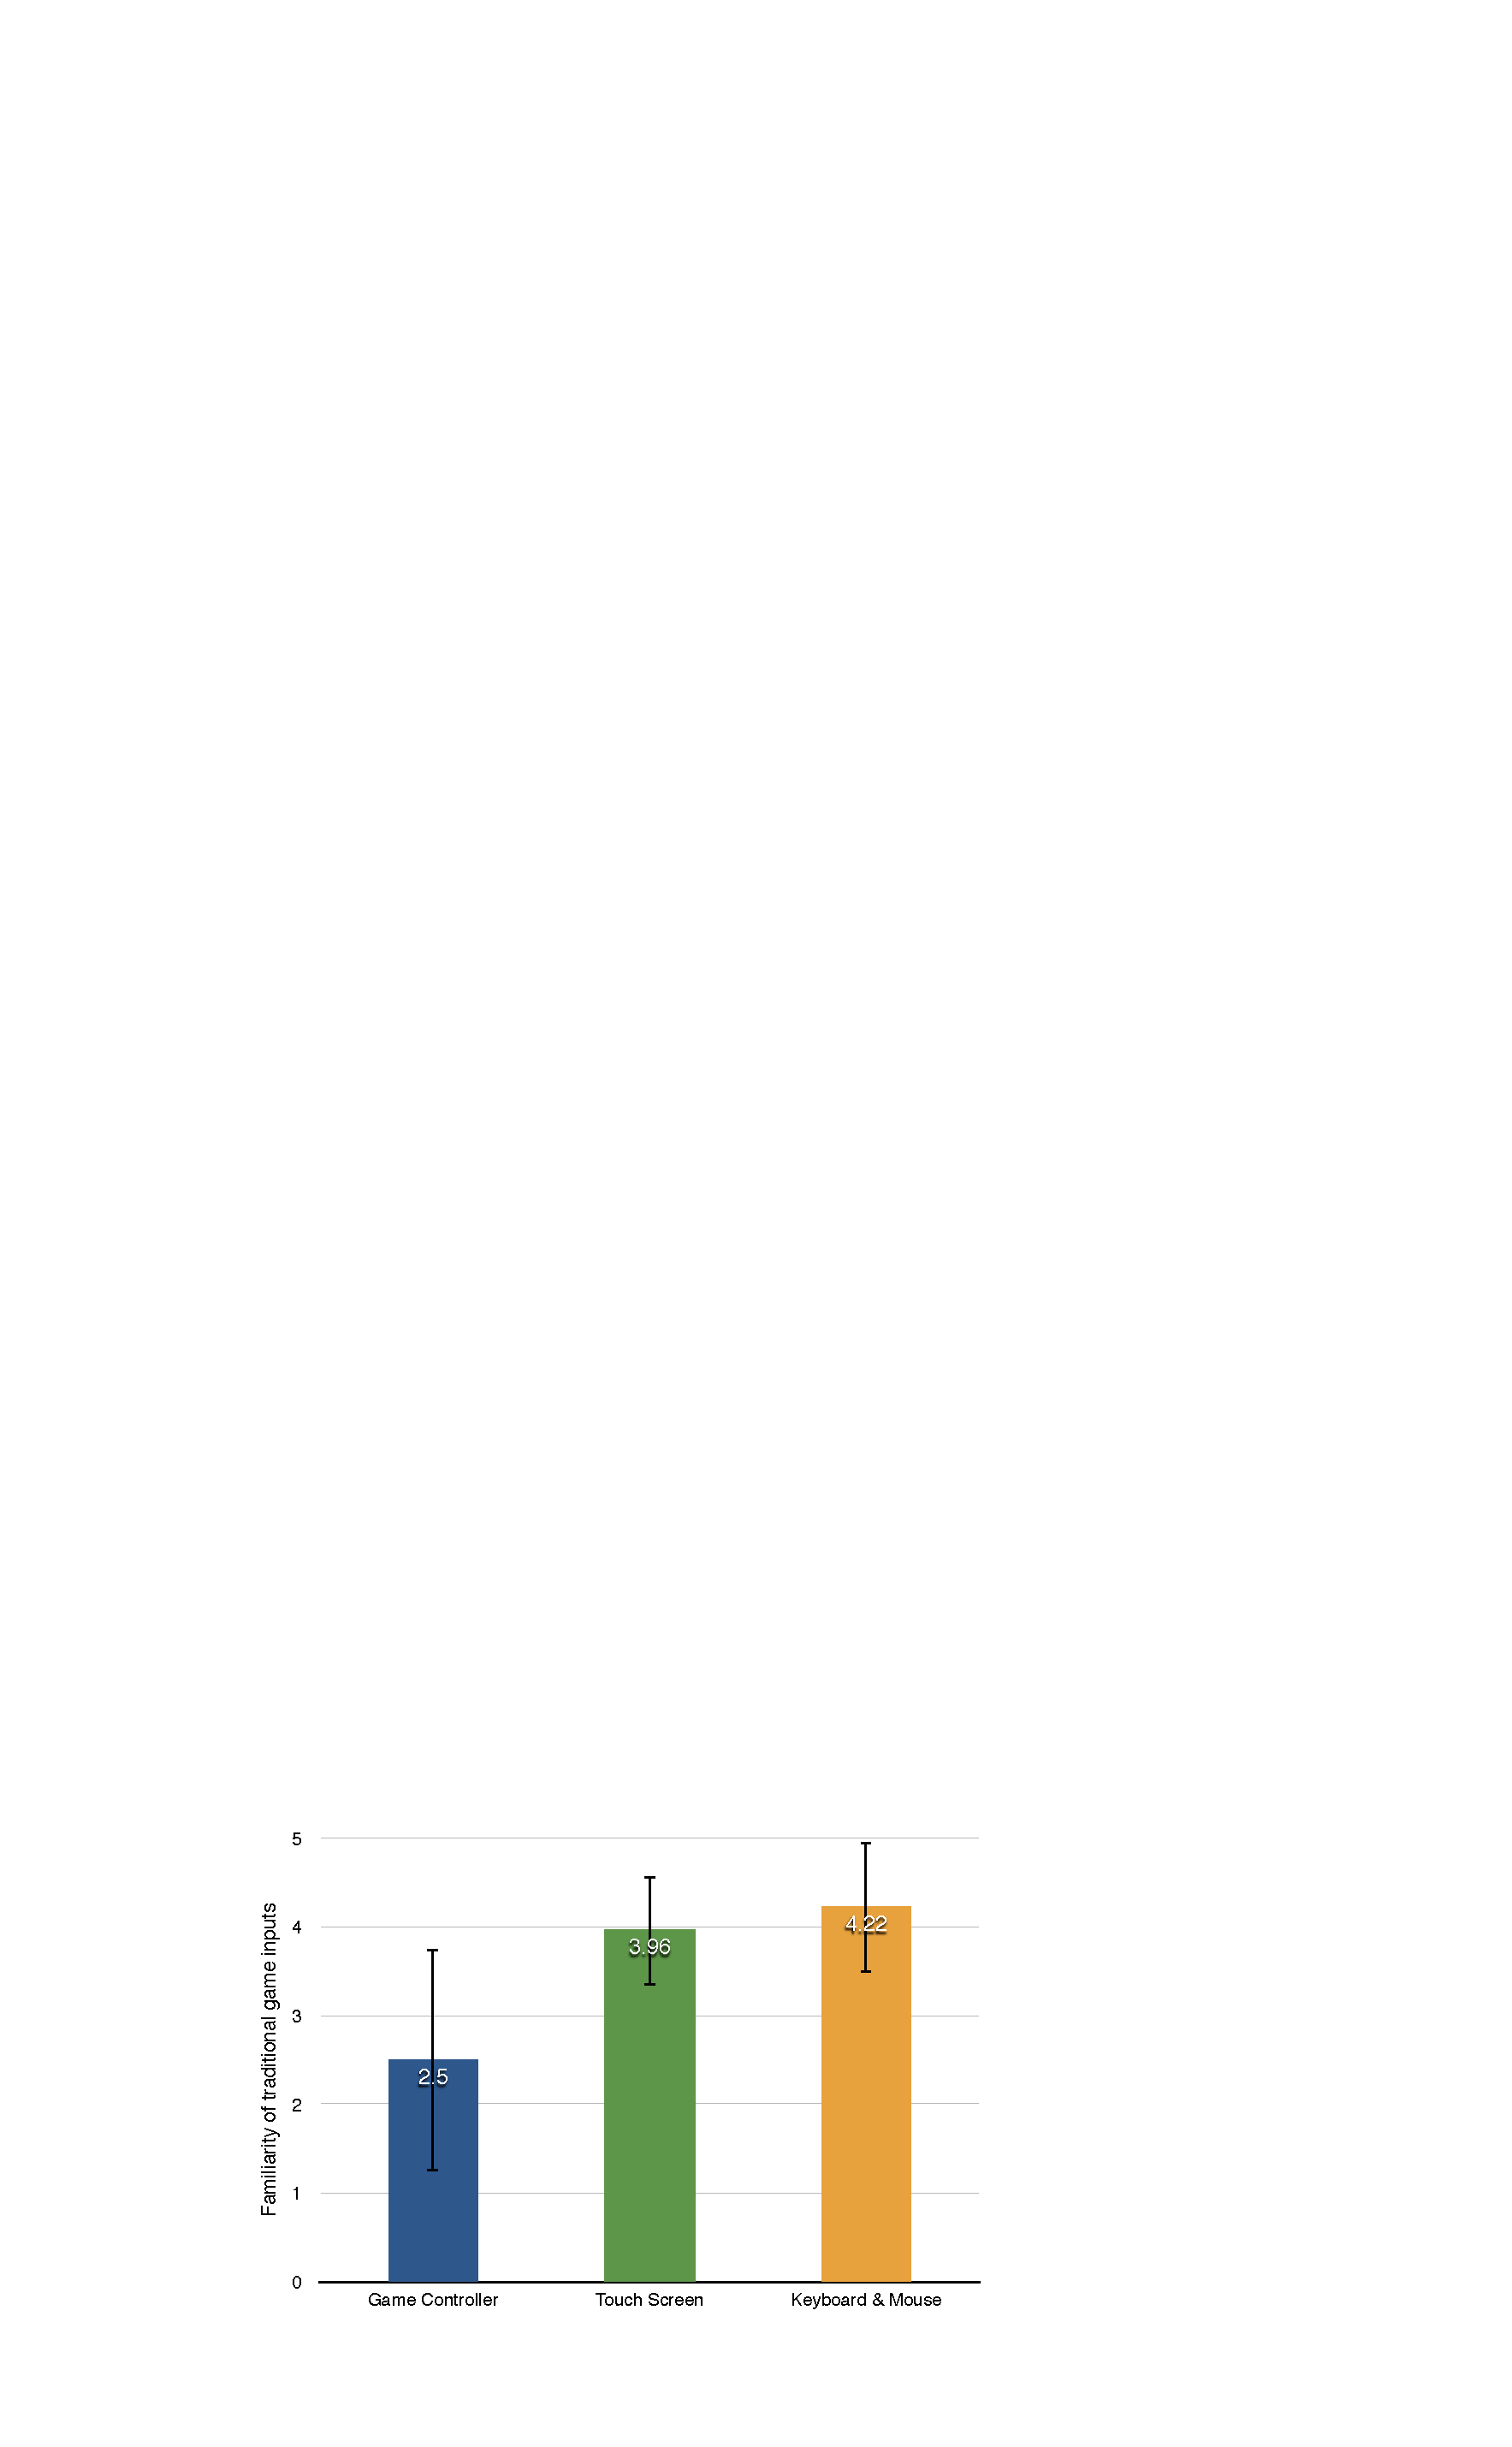
\includegraphics[width=0.8\columnwidth]{Familiarity.pdf}
  %\caption{Users' game input familiarity.}
  %\label{fig:figureFamiliarity}
  %\end{figure}  

  \section {Participants}
  We recruited twenty-four participants with an equal male-female ratio for our study. Their average age was 23.2 (\textsl{sd} = 2.72). All participants are right-handed and none of them had past experience with smart glasses usage. About their gaming experience, according to our investigation, 14 users were daily game players, 9 were weekly players and 1 was a monthly player. Participants spent 1.36 hours (\textsl{sd} = 0.89) on average to play games one time. Moreover, 58\% of them indicated that their main gaming platforms were mobile phones, 38\% were on PCs, and only 4\% were on consoles. Another important factor of the gaming experience is the user's familiarity with game controllers. The results showed that average familiarity scores were 2.50 for gamepad (\textsl{sd} = 1.24), 3.96 for touchscreen (\textsl{sd} = 0.62) and 4.22 for keyboard and mouse (\textsl{sd} = 0.74) on a 5-point Likert Scale for degree of familiarity (1 means very unfamiliar, 5 means very familiar).    


  %compared with a game controller, most of them were more familiar with keyboards, mouses and touch screens (see Figure~\ref{fig:figureFamiliarity}).
  %\begin{figure}[!h]
  %\centering
  %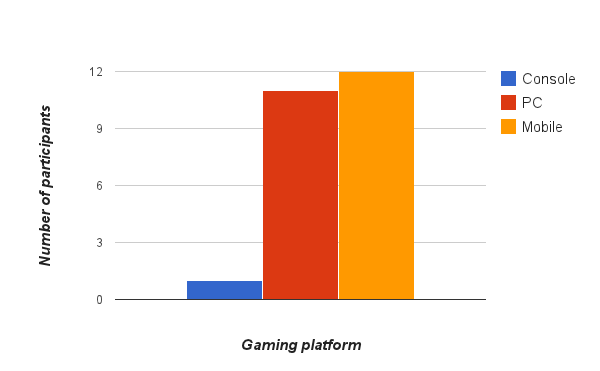
\includegraphics[width=0.9\columnwidth]{Platform}
  %\caption{With Caption Below, be sure to have a good resolution image
  %  (see item D within the preparation instructions).}
  %\label{fig:figurePlatform}
  %\end{figure} 
  %\begin{figure}[!h]
  %\centering
  %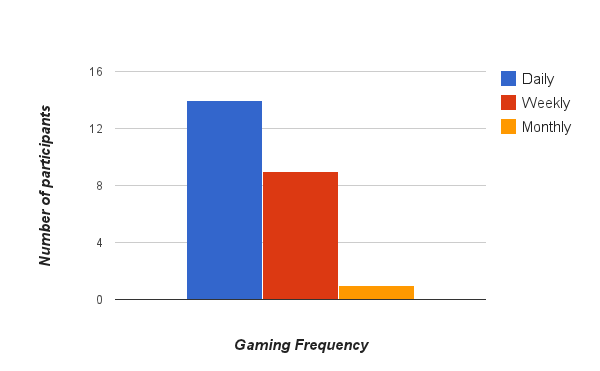
\includegraphics[width=0.9\columnwidth]{Frequency}
  %\caption{With Caption Below, be sure to have a good resolution image
  %  (see item D within the preparation instructions).}
  %\label{fig:figureFrequency}
  %\end{figure}
 

  \section {Environment}
  According to the previous works\cite{Williamson:2013:MEM:2522848.2522874,Montero:2010:YUS:1851600.1851647}, the social acceptability of mobile-input was influenced by whether participants believed a bystander could interpret the intention of the input action. Therefore, to provide a game input set suited for a real-world environment, we chose a Starbucks cafe near our college. The visitor flow of the cafe, on average, was 72.5 persons per hour. In our investigation, participants indicated that the cafe was comparatively a public space with average 4.17 points (\textsl{sd}=0.65) on a 5-point Likert Scale for degree of field publicity (1 means very private, 5 means very public).    

  

    \section {Procedure}
    Participants wore two different glasses (Google Glass and Epson Moverio) and our software randomly presented 17 game tasks (Table \ref{tab:table1}) to participants. For each game task, participants performed an input action in 3 different interaction methods (\emph{handheld}, \emph{touch} and \emph{non-touch} interaction). The study was conducted using a counterbalanced measures design, alternating the glass's form and the interaction method. After each game input, participants were shown a 5-point Likert scale concerning subjective preference and conducted a short interview about input detail. With 24 participants, 17 game tasks, 2 glass forms and 3 interaction methods, a total of $24 \times 17 \times 2 \times 3$ = 2448 game input actions were made. 